\newcommand{\todoroman}[1]{{\color{purple}TODO: #1}}

\newcommand{\comseb}[1]{{\color{red}\footnote{\color{red}Seb: \textit{#1}}}}
\newcommand{\comroman}[1]{{\color{purple}\footnote{\color{purple}Roman: \textit{#1}}}}
\newcommand{\commanu}[1]{{\color{teal}\footnote{\color{teal}Manu: \textit{#1}}}}
\newcommand{\commanue}[1]{{\color{blue}\footnote{\color{blue}Manue: \textit{#1}}}}
\newcommand{\comloic}[1]{{\color{orange}\footnote{\color{orange}Loïc: \textit{#1}}}}

\newcommand{\marquepage}{\noindent{\color{violet}Manue, tu t'es arrêtée de lire ici la dernière fois.}\\\begin{center}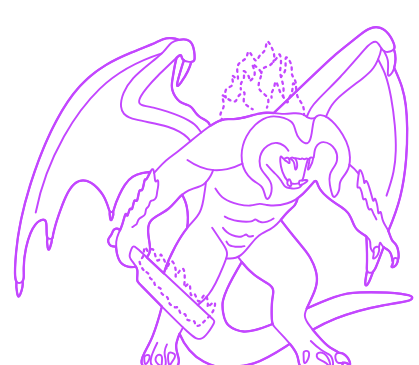
\includegraphics[width=5cm]{tmp/balrog.png}\end{center}}
\newcommand{\youshallnotpass}{\noindent{\color{purple}Attention Manue je m'en suis arrêté là :)}\begin{center}
\includegraphics[width=5cm]{tmp/gandalf.png}\end{center}}

Chapitre 3
Intro
\comloic{n'essaie pas de me le vendre Roman, sort ta machette non stérilisée je suis prêt c'est bon}
\comloic{alors là autant te dire ue j'aime autant parce que j'en viens et j'espère que c'était utile ^^'}

Conclusion
\commanue{Alors quoi ? pas de conclusion ? C'est quoi cette fin de chapitre digne d'un vieux téléfilm sur france 3. Il faut résumer les éléments clés du chapitre et donner envie à ton lecteur qui vient de subir une épreuve de continuer.}
\comloic{alors le chapitre 3, pour moi, c'est écouter Carole essayer de me raconter un truc qui semble lui paraitre super important, et me perdre dans la définition énorme d'un contexte dont je ne saisis plus la partie essentielle faute d'avoir eu une idée de la violence avec laquelle le sujet allait me percuter dans un avenir proche. Si bien que à la fin, je me sens mal à l'aise devant le gap qui sépare ce que j'ai cru comprendre et l'émotion qui se traduit sur son visage. Un peu comme si elle venait de livrer une conclusion qui, dans mon référentiel, pourrait tout aussi bien avoir été l'introduction ou une parenthèse. Par exemple, ici, j'ai tout à fait l'impression que j'ai du passer à côté de la conclusion parce que je ne m'attendais pas du tout à ce que tu cesses de parler après l'exemple 13. Pour te dire j'attendais le 3.3 depuis quelques paragraphes, où, à la manière de David Fincher, tu allais recoler en une phrase claire et limpide comme destinée à un enfant l'ensemble des éléments vus précédemment, et tout allait prendre forme dans ma tête durant les 2h prochaines heures. Honnêtement je me sentais bien durant le 3.1. Mais le 3.2 je l'ai subie. J'ai perdu de vu le sommet du Tourmalet et je n'ai pas cessé de me demander si j'étais encore sur la bonne route. "Allez Loïc tu vois bien que c'est la route principale". "Ouais mais imagine... imagine on pédale pour rien... on n'a pas de GPS rien que dalle". Ce sont les commentaires de Manue qui m'ont convaincu de m'accrocher un peu, comme pour dire "allez, moi aussi j'ai fait l'effort". En gros j'ai compris qu'il y avait un truc sur les inclusions entre les trois méthodes du 3.1. Mais au fur et à mesure j'ai eu le sentiement de perdre espoir. J'avais l'impression qu'à chaque fois on me présentait de nouveaux concepts qui finissaient par un constat défaitiste. Est ce qu'on a réussi à trouver un scénario favorable qui nous aide à calculer notre copula simplement tout en pouvant dire qu'elle inclue dans la meilleure des copulas alors que c'est la copule la plus simple à calculer ? Est ce qu'on va pouvoir s'en sortir Roman ? Bon je vais voir le chapitre 4 j'aurai peut être ma réponse ^^.}\comloic{dernier petit point, est ce qu'on peut argumenter que ton apport sur le chapitre 3, ton travail de thèse, consiste en toutes les propositions que tu démontres ici (sous entendu parce qu'elles ne seraient pas démontrées dans un papier préalable à ta thèse ?). J'ai parfois eu du mal à cerner ce qui était nouveau pour un lecteur compétent.}


Chapitre 4
\comloic{tu n'imagines pas le bonheur que je ressens à l'orée de ce chapitre 4 (puis 5), c'est comme sortir d'une forêt obscure, rentrer à la maison et retrouver des odeurs communes, comme si plus rien ne pouvait arriver qui nous surprenne, c'est retrouver la serrenite, l'impression d'être à l'heure} 
\comloic{et là c'est le moment où tu comprends qu'il y a une continuité entre la forêt obscure et la maison, comme si tu n'étais pas rentré tout seul de là bas}

\commanue{oh mon dieu une conclusion, j'ai pas l'habitude, peut-être faire une section dédiée, c'est toi qui voit}

\comloic{le retour de la remark qui tue. Ce "Remark" en gras il me donne la chair de poule mnt ^^' Dis toi que le lecteur qui découvre, il est concentré sur ta mesure d'ambiguité que tu viens de citer plus haut. Et tout à coup c'est une pub que tu l'envoies. Il change de sujet, il a envie de zapper la remarque mais en même temps l'ayant lue de travers pour ne pas perdre le fil il se dit "attends quoi? c'est quoi cette subtilité qu'on vient de me faire avaler l'air de rien?". C'est vraiment comme annoncer entre la dinde et le dessert qu'une partie des champignons utilisés pour le velouté en entrée étaient peut être périmés mais tu penses avoir enlever le plus mauvais. "Et voilà la tarte aux pommes maison! Régalez vous !" }
\comloic{c'était peut être vrai pour le papier mais là tu dis ça à des gens qui sont passés par les chapitres 2 et 3 quand même... c'est un peu mesquin de ta part}

\commanue{donc tu as des synonymes pour ton mot favori consider en fait ;)}

\comloic{peut être que c'est une autre façon de dire que le choix du alpha doit se faire par estimateur de similarité. Tu précises, forte heureusement, plus haut, que le alpha=0.9 n'est pas en lien avec l'objectif de 90 pour cent mais on ne précise pas vraiment que pour atteindre 90/100 il n'y a pas de raison de croire que la même valeur de alpha soit la bonne pour deux mesures de similarité différente. Et que donc partout qd tu compares les intervalles MCCNN et Census, c'est à MCCNN à alpha=0.9 et Census à alpha=0.9. D'autant que chacune des mesures a aussi j'imagine des zones de faible confiance différentes ce qui est un autre impact majeur sur l'interprétation, et surtout la comparaison des orel. Rien ne dit qu'on doivent paramétrer l'ambiguité de la même façon pour les deux mesures etc. Donc bon en gros attention juste peut être à ne pas graver dans le marbre des choses qui dépendent de nombreux hyperparamètres. J'en suis presque à dire qu'il manque une remarque. Incroyable ^^. Non je déconne, mais peut être un préambule quelque part.}.

\comloic{sleeper slopes ? vivement la fin de la thèse il te manque un peu de sommeil non ? ;-)}

\commanu{quid également de mettre un mot sur le fait que tu fais de l'IA aussi et que pas obligé de faire du deep learning pour etre funky et à la page :) }